\begin{figure}[ht]\centering
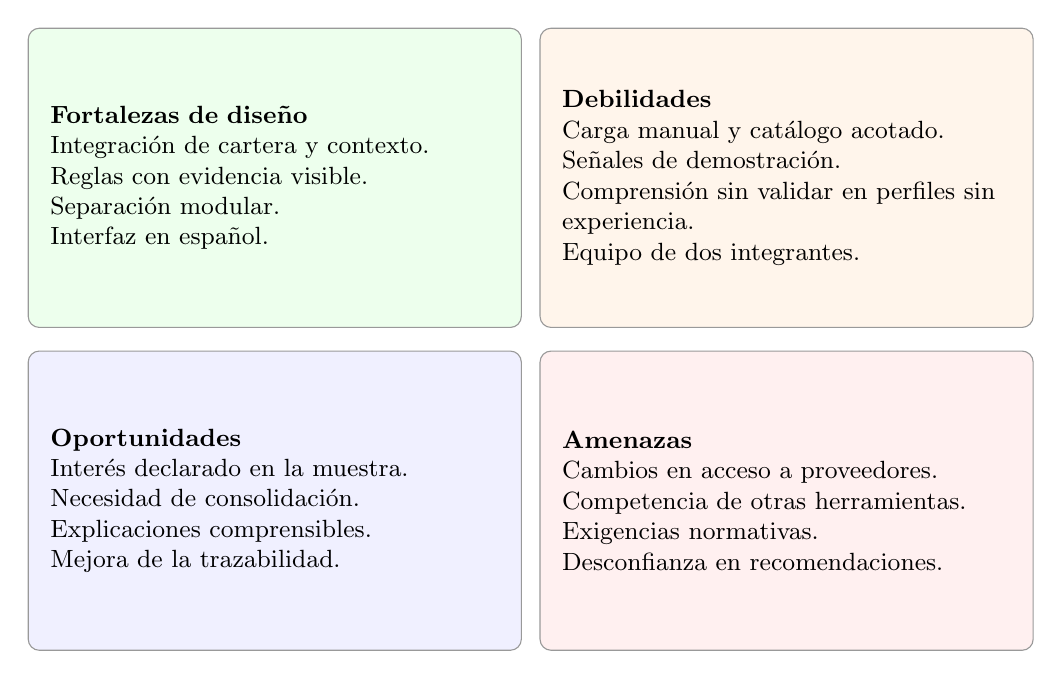
\begin{tikzpicture}[q/.style={draw=black!40,rounded corners,text width=5.7cm,minimum height=3.8cm,align=left,inner sep=8pt,font=\small,anchor=north west}]
\node[q,fill=green!7] at (0,0) {\textbf{Fortalezas de diseño}\\Integración de cartera y contexto.\\Reglas con evidencia visible.\\Separación modular.\\Interfaz en español.};
\node[q,fill=orange!8] at (6.5,0) {\textbf{Debilidades}\\Carga manual y catálogo acotado.\\Señales de demostración.\\Comprensión sin validar en perfiles sin experiencia.\\Equipo de dos integrantes.};
\node[q,fill=blue!6] at (0,-4.1) {\textbf{Oportunidades}\\Interés declarado en la muestra.\\Necesidad de consolidación.\\Explicaciones comprensibles.\\Mejora de la trazabilidad.};
\node[q,fill=red!6] at (6.5,-4.1) {\textbf{Amenazas}\\Cambios en acceso a proveedores.\\Competencia de otras herramientas.\\Exigencias normativas.\\Desconfianza en recomendaciones.};
\end{tikzpicture}
\caption{Análisis FODA del Proyecto. Fuente: elaboración propia.}\label{fig:foda}
\end{figure}
